% LaTeX resume using res.cls
\documentclass[line,margin]{res} 
%\usepackage{helvetica} % uses helvetica postscript font (download helvetica.sty)
%\usepackage{newcent}   % uses new century schoolbook postscript font 

\usepackage[utf8]{inputenc}
\usepackage[norsk]{babel}

\newcommand{\zh}{Z\"{u}rich}
\usepackage{charter}
\usepackage{graphicx}
\usepackage{wrapfig}

\begin{document}

\name{Eivind Fonn}
% \address used twice to have two lines of address
\address{Forchstrasse 168, CH-8032 \zh}
\address{+41 78 634 68 37, evfonn@gmail.com}


\begin{resume}

\section{PERSONALIA}
    \begin{wrapfigure}{R}{0.13\textwidth}
        \vspace{-0.6cm}
        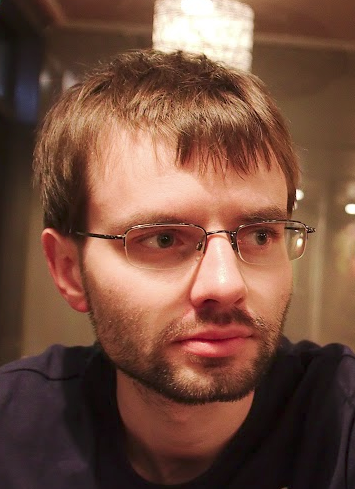
\includegraphics[width=1.5cm]{photo.png}
    \end{wrapfigure}
    Jeg er en ugift 29 år gammel nordmann, født, oppvokst og studert i Trondheim. Jeg flyttet til \zh,
    Sveits for doktorgradsstudier. Interessert i matematikk, numerikk, programmering, fotografi, sjakk og
    bøker generelt.


\section{UTDANNING} 
    {\em Doktorgrad}, anvendt matematikk \hfill 2009-09 $\to$ 2013-11 \\
    ETH \zh, \zh, Sveits \\
    Løsning av høydimensjonale kinetiske transportligner, for å bekjempe
    ``dimensjonalitetsforbannelsen''. Spesielt fokus på shearlet\-rammer og
    Boltzmann\-ligningen.

    {\em Siv. ing.}, industriell matematikk \hfill 2004-08 $\to$ 2009-06 \\
    NTNU, Trondheim, Norge \\
    Spesialisering i numerisk analyse, geometrisk integrasjon og differensialgeometri


\section{FERDIGHETER}
    {\em Programmering:} Python, Matlab, Haskell, C, C++, C$\sharp$, Java, PHP, JS \\
    {\em Databaser:} PostgreSQL, MySQL, MS SQL \\
    {\em Div. data:} \LaTeX, (X)HTML, CSS, XML \\
    {\em Operativsystemer:} Diverse Linuxdistribusjoner, Windows \\
    {\em Språk:} Flytende norsk og engelsk, brukbar tysk


\section{ERFARING} 
    {\em Doktorgradsstudent} \hfill 2009-09 $\to$ 2013-11 \\
    ETH \zh, \zh, Sveits \\
    Løsning av høydimensjonale kinetiske transportligner, for å bekjempe
    ``dimensjonalitetsforbannelsen''. Implementasjon i Matlab, Python og C.
    Inkluderer en undervisningsandel på 40\%.

    {\em Programmerer} \hfill Sommeren 2009 \\
    Jeeves, Trondheim, Norge \\
    Implementerte et over\-settings\-verktøy bygd på Google Translate, som
    kan lese og skrive et antall forskjellige formater (deriblant Microsoft
    Word og databasetabeller), men funksjonalitet for å huske spesialfraser
    og rettelser av feil\-over\-settinger.

    {\em Programmerer} \hfill Sommeren 2008 \\
    Yahoo! Technologies, Trondheim, Norge \\
    Implementerte et adapter mellom MySQL og Yahoos interne vertikale 
    søke\-plat\-form Vespa, med flere demoer. Ansvar for hele prosessen, fra
    design til fullføring.

    {\em Vitenskapelig assistent} \hfill Sommeren 2007 \\
    ETH \zh, \zh, Sveits \\
    Implementerte en endelig volum\-metode for å løse en modell for konveksjon,
    diffusjon og reaksjon i Matlab. Gjorde også post\-prosessering av simu\-leringer
    for foton\-krystaller. IAESTE-utplas\-sering.


\section{PRISER}
    \begin{itemize}
        \item Winnie og Ragnar Mathisens pris for beste student på siv. ing. 
            eller arkitekt på NTNU i 2009.
        \item Norsk Regnesentrals pris for beste masteroppgave i matematikk
            eller IKT på NTNU i 2009.
        \item Stubbanprisen for mest lovende masterkandidat i matematikk på
            NTNU i 2009.
    \end{itemize}


\section{DIVERSE}
    \begin{itemize}
        \item Grunnleggeren av Aligulac-prosjektet\footnote{{\tt http://aligulac.com/}}, 
            et ratingsystem og en historisk database for profesjonell StarCraft 2, nå
            drevet av et team på rundt 15 frivillige.
        \item Delarrangør av den første utgaven av KoMiN---en årlig konferanse for
            matematikkstudenter i Norge.
        \item Lagde oppgaver, rettet svar og vedlikeholdt nettsiden for Abelkonkurransen.
        \item Drivkraften og hovedarrangør for de to første utgavene av NM i Rubiks kube.
        \item Tidligere norsk rekordholder i Rubiks kube hurtigløsning, vanlig og i blinde.
    \end{itemize}


\section{TILLITSVERV}
    \begin{itemize}
        \item Webmaster\footnote{{\tt http://iaeste.ch/}} og styremedlem for IAESTEs
            lokalkomité i \zh i fire år (2010-2013).
        \item Anerkjent av verdens kubeforening (WCA) som offentlig konkurransedelegat.
        \item Webmaster og styremedlem i linjeforeninge Nabla på NTNU i tre år
            (2005-2007).
    \end{itemize}


\section{REFERANSER}
    \begin{itemize}
        \item Prof. Dr. Ralf Hiptmair, Seminar for Applied Mathematics, ETH Zurich \\
            +41 44 632 34 04, ralf.hitpmair@sam.math.ethz.ch
        \item Prof. Dr. Philipp Grohs, Seminar for Applied Mathematics, ETH Zurich \\
            +41 44 632 32 00, philipp.grohs@sam.math.ethz.ch
    \end{itemize}


\section{SOSIALE NETTVERK}
    \begin{itemize}
        \item Github: \texttt{http://github.com/TheBB}
        \item LinkedIn: \texttt{http://www.linkedin.com/pub/eivind-fonn/5/364/67}
    \end{itemize}


\end{resume}
\end{document}
